\section{Exposition of Languages and Equivalence Definition}
\label{sec:lang-eqdef}

\subsection{The \SpecL{} Language}
\label{sec:speclang}
We start with a discussion on the \SpecL{} language.
\SpecL{} supports recursive algebraic data types (ADT) similar to the ones available in most functional languages.
Additionally, \SpecL{} is equipped with the following scalar types: \type{Unit}, Boolean (\type{Bool}) and Bitvector of length N (\type{i<N>}).
ADTs can be thought of as `sum of product' types where each constructor represents a variant
and the arguments to each constructor represents its fields.
Evidently, types in \SpecL{} can be represented in {\em first order recursive types} with {\tt Product} and {\tt Sum} type constructors and {\tt Unit, Bool, i<N>} types (i.e., nullary type constructors) as follows:

$T \rightarrow {\tt \mu} \alpha.\ T \ |\  {\tt Product}(T,\dots,T) \ |\  {\tt Sum}(T,\dots,T) \ |\  {\tt Unit} \ |\ {\tt Bool} \ |\  {\tt i\langle N \rangle} \ |\  \alpha$

For example, the {\tt List} type can be written as $\mu \alpha. Sum(Unit, Product(i32,\alpha))$.

The language also borrows its expression grammar heavily from functional languages.
This includes the usual constructs like {\tt let-in}, {\tt if-then-else}, function application and the {\tt match} statement
for pattern-matching (i.e. deconstructing) sum and product values.
Unlike functional languages, \SpecL{} only supports first order functions.
Also, \SpecL{} does not support partial function application.
Hence, we constrain our attention to C programs containing only first order functions.
\SpecL{} is equipped with a special {\tt assuming-do} construct for explicitly providing assertions.
\SpecL{} also provides the typical boolean and bitvector operators for expressing computation in C succintly yet explicitly.
This includes logical operators (e.g., {\tt and}), bitvector arithmatic operators (e.g., {\tt bvadd(+)}) and
relational operators for comparing bitvectors interpreted as signed or unsigned integers (e.g., {\tt $\leq_{u,s}$}).

\begin{figure}[H]
\begin{small}
\begin{tabular}{rcl}
\nonTerm{expr} & $\rightarrow$ & \term{if} \nonTerm{expr} \term{then} \nonTerm{expr} \term{else} \nonTerm{expr} \\
& $|$ & \term{let} \nonTerm{id} \term{=} \nonTerm{expr} \term{in} \nonTerm{expr} \\
& $|$ & \term{match} \nonTerm{expr} \term{with} \nonTerm{match-clause-list} \\
& $|$ & \term{assuming} \nonTerm{expr} \term{do} \nonTerm{expr} \\
& $|$ & \nonTerm{id} \term{(} \nonTerm{expr-list} \term{)} \\
& $|$ & \nonTerm{data-cons} \term{(} \nonTerm{expr-list} \term{)} \\
& $|$ & \nonTerm{expr} \term{is} \nonTerm{data-cons} \\
& $|$ & \nonTerm{expr} \nonTerm{scalar-op} \nonTerm{expr} \\
& $|$ & \nonTerm{literal$_{\mathrm{Unit}}$} $|$ \nonTerm{literal$_{\mathrm{Bool}}$} $|$ \nonTerm{literal$_{\mathrm{i<N>}}$} \\
\\
\nonTerm{match-clause-list} & $\rightarrow$ & \nonTerm{match-clause}$^*$ \\
\nonTerm{match-clause} & $\rightarrow$ & \term{$|$} \nonTerm{data-cons} \term{(} \nonTerm{id-list} \term{)} \term{$\Rightarrow$} \nonTerm{expr} \\
\nonTerm{expr-list} & $\rightarrow$ & \term{$\epsilon$} \term{$|$} \nonTerm{expr} \term{,} \nonTerm{expr-list} \\
\nonTerm{id-list} & $\rightarrow$ & \term{$\epsilon$} \term{$|$} \nonTerm{id} \term{,} \nonTerm{id-list} \\
\\
\nonTerm{literal$_{\mathrm{Unit}}$} & $\rightarrow$ & \term{()} \\
\nonTerm{literal$_{\mathrm{Bool}}$} & $\rightarrow$ & \term{false} $|$ \term{true} \\
\nonTerm{literal$_{\mathrm{i<N>}}$} & $\rightarrow$ & [\term{0$\dots$2$^{\mathrm{N}}$-1}] \\
\end{tabular}
\end{small}
\caption{\label{fig:specgrammar}Simplified expression grammar of \SpecL{} language}
\end{figure}

\subsection{Intermediate Representations}
\label{sec:ir}
As summarized in \cref{sec:summary}, we lower both \SpecL{} and C programs to a common
intermediate representation (IR) for comparison.
IR is a Three-Address-Code (3AC) style intermediate representation.
We often omit intermediate registers in the IR for brevity and ease of exposition,
and refer to this as the {\em abstracted} IR.

\begin{figure}
\begin{tabular}{cc}
\begin{subfigure}[b]{0.45\textwidth}
\begin{center}
\begin{allLangEnvFoot}
~{\scriptsize \textcolor{mygray}{   }}~   
~{\scriptsize \textcolor{mygray}{S0:}}~ i32 sum_list (List l) {
~{\scriptsize \textcolor{mygray}{S1:}}~   i32 sum $\coloneqq$ ${\tt 0_{i32}}$;
~{\scriptsize \textcolor{mygray}{S2:}}~   while $\mathrm{\tt\neg (l\ is\ LNil)}$:
~{\scriptsize \textcolor{mygray}{S3:}}~     // (l is LCons);
~{\scriptsize \textcolor{mygray}{S4:}}~     sum $\coloneqq$ sum + ${\tt l.val}$;
~{\scriptsize \textcolor{mygray}{S5:}}~     l   $\coloneqq$ l.next;
~{\scriptsize \textcolor{mygray}{S6:}}~   return sum;
~{\scriptsize \textcolor{mygray}{SE:}}~ }
\end{allLangEnvFoot}
\end{center}
\caption{\label{fig:llTraverseSpec}(Abstracted) Spec IR}
\end{subfigure}%
&
\begin{subfigure}[b]{0.55\textwidth}
\begin{center}
\begin{allLangEnvFoot}
~{\scriptsize \textcolor{mygray}{\ \ \ }}~ unsigned sum_list (lnode* l);
~{\scriptsize \textcolor{mygray}{C0:}}~ i32 sum_list (i32 l) {
~{\scriptsize \textcolor{mygray}{C1:}}~   i32 sum $\coloneqq$ ${\tt 0_{i32}}$;
~{\scriptsize \textcolor{mygray}{C2:}}~   while ${\tt l \neq 0_{i32}}$:
~{\scriptsize \textcolor{mygray}{C3:}}~     sum $\coloneqq$ sum + $\structPointer{\tt l}{m}{\tt lnode}{val}$;
~{\scriptsize \textcolor{mygray}{C4:}}~     l   $\coloneqq$ $\structPointer{\tt l}{m}{\tt lnode}{next}$;
~{\scriptsize \textcolor{mygray}{C5:}}~   return sum;
~{\scriptsize \textcolor{mygray}{CE:}}~ }
\end{allLangEnvFoot}
\end{center}
\caption{\label{fig:llTraverseC}(Abstracted) C IR}
\end{subfigure}%
\\
\begin{subfigure}[b]{0.45\textwidth}
\begin{center}
{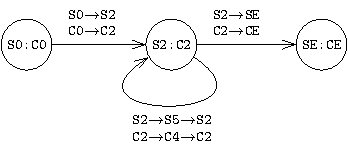
\includegraphics[scale=1.1]{chapters/figures/figSumListProductCfg.pdf}}
\end{center}
\caption{\label{fig:llTraverseProduct}Product-CFG}
\end{subfigure}%
&
\begin{subfigure}[b]{0.55\textwidth}
\begin{center}
\begin{footnotesize}
\begin{tabular}{|c|l|}
\hline
\tt PC-Pair & \multicolumn{1}{c|} {\tt Invariants} \\
\hline
\hline
${\tt (S0:C0)}$ &
\Tstrut ${\tt {\circled{P}}\  l_{S}\indEq{}Clist^{lnode}_{m}(l_{C})}$ \\
\multirow{2}{*}{${\tt (S2:C2)}$} &
\Tstrut \Bstrut ${\tt {\scriptsize \circled{I1}}\  l_{S}\indEq{}Clist^{lnode}_{m}(l_{C})}$ \\ & ${\tt {\scriptsize \circled{I2}}\  sum_{S}=sum_{C}}$ \\
${\tt (SE:CE)}$ &
\Tstrut \Bstrut ${\tt {\circled{E}}\  ret_{S}=ret_{C}}$ \\
\hline
\end{tabular}
\end{footnotesize}
\vspace{13px}
\end{center}
\caption{\label{fig:llTraverseProductInv}Node Invariants of the Product-CFG}
\end{subfigure}%
\\
\end{tabular}
\caption{\label{fig:llTraverseSpecAndC}Spec and C programs for traversing a linked list. \Cref{fig:llTraverseProduct} shows the Product-CFG between the IRs in \cref{fig:llTraverseSpec,fig:llTraverseC}. The inductive invariants of the Product-CFG are given in \cref{fig:llTraverseProductInv}.}
\end{figure}

\begin{figure}
\begin{tabular}{cc}
\begin{subfigure}[b]{0.45\textwidth}
\begin{center}
\begin{allLangEnvFoot}
~{\scriptsize \textcolor{mygray}{S0:}}~ i32 sum_list (List l) {
~{\scriptsize \textcolor{mygray}{S1:}}~   i32 sum $\coloneqq$ ${\tt 0_{i32}}$;
~{\scriptsize \textcolor{mygray}{S2:}}~   while $\neg$(l is LNil):
~{\scriptsize \textcolor{mygray}{S3:}}~     // (l is LCons);
~{\scriptsize \textcolor{mygray}{S4:}}~     sum $\coloneqq$ sum + l.val;
~{\scriptsize \textcolor{mygray}{S5:}}~     l   $\coloneqq$ l.next;
~{\scriptsize \textcolor{mygray}{S6:}}~   return sum;
~{\scriptsize \textcolor{mygray}{SE:}}~ }
\end{allLangEnvFoot}
\end{center}
\caption{\label{fig:llTraverseSpecIR}(Abstracted) Spec IR}
\end{subfigure}%
&
\begin{subfigure}[b]{0.55\textwidth}
\begin{center}
\begin{allLangEnvFoot}
~{\scriptsize \textcolor{mygray}{C0:}}~ i32 sum_list (i32 l) {
~{\scriptsize \textcolor{mygray}{C1:}}~   i32 sum $\coloneqq$ ${\tt 0_{i32}}$;
~{\scriptsize \textcolor{mygray}{C2:}}~   while ${\tt l \neq 0_{i32}}$:
~{\scriptsize \textcolor{mygray}{C3:}}~     sum $\coloneqq$ sum + $\structPointer{\tt l}{\mem{}}{lnode}{val}$;
~{\scriptsize \textcolor{mygray}{C4:}}~     l   $\coloneqq$ $\structPointer{\tt l}{\mem{}}{lnode}{next}$;
~{\scriptsize \textcolor{mygray}{C5:}}~   return sum;
~{\scriptsize \textcolor{mygray}{CE:}}~ }
\end{allLangEnvFoot}
\vspace{7px}
\end{center}
\caption{\label{fig:llTraverseCIR}(Abstracted) C IR}
\end{subfigure}%
\\
\begin{subfigure}[b]{0.45\textwidth}
\begin{center}
{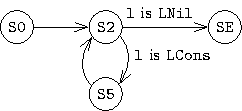
\includegraphics[scale=1.3]{chapters/figures/figSumListSpecCfg.pdf}}
\end{center}
\caption{\label{fig:llTraverseSpecCFG}CFG of \SpecL{} Program}
\end{subfigure}%
&
\begin{subfigure}[b]{0.55\textwidth}
\begin{center}
{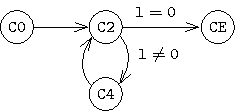
\includegraphics[scale=1.3]{chapters/figures/figSumListCCfg.pdf}}
\end{center}
\caption{\label{fig:llTraverseCCFG}CFG of C Program}
\end{subfigure}%
\\
\end{tabular}
\caption{\label{fig:llTraverseSpecAndCIRAndCFG}IRs and CFGs of the \SpecL{} and C Programs in \cref{fig:llTraverseSpec,fig:llTraverseC} respectively.}
\end{figure}


\Cref{fig:llTraverseSpec,fig:llTraverseC} show \SpecL{} and C programs that traverse a linked list
and return the sum of all the values in the linked list.
The corresponding IR programs are shown in \cref{fig:llTraverseSpecIR,fig:llTraverseCIR}.

During conversion of a \SpecL{} source (\cref{fig:llAllocSpec,fig:llTraverseSpec} resp.)
to IR (\cref{fig:llAllocSpecIR,fig:llTraverseSpecIR} resp.),
(a) {\tt match} statements are lowered to explicit \sumDtor{} conditionals where each branch
represents a distinct constructor,
(b) all tail-recursive calls are converted to loops while non-tail calls are preserved and
(c) all helper functions are inlined at their call-site.

Similarly, the following is performed during conversion of a C source (\cref{fig:llAllocC,fig:llTraverseC} resp.)
to IR (\cref{fig:llAllocCIR,fig:llTraverseCIR} resp.):
(a) the sizes and memory layouts of both scalar (e.g., \type{unsigned})
and compound (e.g., \type{struct lnode}) types are concretized,
(b) the program memory along with reads and writes to it are made explicit and
(c) we annotate {\tt malloc} calls with the call-site
i.e. IR PC (e.g., {\tt malloc$_\cpc{4}$} in \cref{fig:llAllocCIR}).

The IR supports both scalar and ADT types available in \SpecL{}.
Each ADT value is modeled as a key-value dictionary that maps
each of its field names to the constituent values.
These key-value pairs are accessed using the {\em accessor}-operator,
e.g., \prodAccess{l}{val} and \prodAccess{l}{next} represents the first and second
fields of the \cons{LCons} constructor in \cref{fig:llTraverseSpecIR}.
The IR also allows querying the top-level value constructor of an ADT value
using the {\em is}-operator, e.g., \sumIs{l}{LNil} in \cref{fig:llTraverseSpecIR}.
Importantly, $l.val$ is only well-formed if \sumIs{l}{LCons}.
The construction of the \SpecL{} IR ensures the well-formedness of all expressions.
Using the {\em accessor}- and {\em is}-operators, a \type{List} value $l$ can be expanded as:

\begin{equation}
\label{eqn:specDeconstruct}
U_S: l = \sumIf{\sumIs{l}{LNil}} \  \sumThen{\cons{LNil}} \  \sumElse{\cons{LCons}(\prodAccess{l}{val}, \prodAccess{l}{next})}
\end{equation}

In this expanded representation of $l$,
the {\em sum-deconstruction} operator `\sumDtor{}'
\footnote{The sum-deconstruction operator `\sumDtor{}' for an ADT
type $T$ must contain exactly one branch for each top-level value constructor of $T$.
For example, `\sumDtor{}' for the \type{List} type must have exactly two branches
of the form \cons{LNil} and $\cons{LCons}(e_1,e_2)$ for some expressions $e_1$ and $e_2$.}
conditionally deconstructs the sum type into its variants \cons{LNil} and \cons{LCons}.
\Cref{eqn:specDeconstruct} is called the {\em unrolling procedure} for the \type{List} variable $l$.
We can similarly define the unrolling procedure for any ADT variable.

The C memory is modeled as a byte-addressable array \mem{} in the IR.
Memory reads are represented using the following two C-like syntaxes:
(a) ``\structPointer{p}{\mem{}}{T}{f}'' is equivalent to ``*(\typeof{T.f}*)(\&\mem{}[$p$+\offsetof{T}{f}])''
i.e., it returns the bytes in the memory array \mem{} starting at address `$p$+\offsetof{T}{f}'
and interpreted as an object of type `\typeof{T.f}' and
(b) ``\arrIndex{p}{i}{\mem{}}{T}'' is equivalent to ``*(T*)(\&\mem{}[$p+i\times$\sizeof{T}])''
i.e., it returns the bytes in the memory array \mem{} starting at address `$p+i\times$\sizeof{T}'
and interpreted as an object of type `\type{T}'.
``\memWrite{\mem{}}{a}{v}{T}'' represents an array that is equal to \mem{} everywhere except at addresses
[$a$, $a$+\sizeof{T}) which contains the value $v$ of type `\type{T}'.

\Cref{fig:llTraverseSpecCFG,fig:llTraverseCCFG} show the Control-Flow Graph (CFG) representation
of the \SpecL{} and C IRs in \cref{fig:llTraverseSpecIR,fig:llTraverseCIR} respectively.
Each CFG node represents a IR PC location of the program and edges represent
transitions through execution of instructions.
Each edge is associated with
(a) a {\em edge condition} (the condition under which that edge is taken),
(b) a {\em transfer function} (how the program state is mutated if that edge is taken) and
(c) a {\em UB assumption} (what condition should be true for the program execution
to be well-defined across this edge).
In \SpecL{}, assertions expressed using the {\tt assuming-do} statement
form the UB assumptions.
For brevity, we often represent a sequence of instructions with a single edge, e.g.,
in \cref{fig:llAllocCCFG}, the edge \cpath{5,3} represents the path \cpath{5,6,7,8,3}.
In such a case, the transfer function of the edge is the composition of the sequence of instructions.


\begin{figure}
\begin{tabular}{cc}
\begin{subfigure}[b]{0.45\textwidth}
\begin{center}
{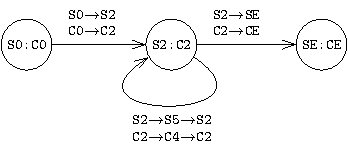
\includegraphics[scale=1.1]{chapters/figures/figSumListProductCfg.pdf}}
\end{center}
\caption{\label{fig:llTraverseProduct}Product-CFG}
\end{subfigure}%
&
\begin{subfigure}[b]{0.55\textwidth}
\begin{center}
\begin{footnotesize}
\begin{tabular}{|c|l|}
\hline
{\bf PC-Pair} & \multicolumn{1}{c|} {\bf Invariants} \\
\hline
\hline
(\scpc{0}{0}) &
\Tstrut $\circled{P}\  \sv{l} \indEq{} \lifted{list}{\mem{}}{lnode}{\cv{l}}$ \\
\multirow{2}{*}{(\scpc{2}{2})} &
\Tstrut $\circled{\scriptsize I1}\  \sv{l} \indEq{} \lifted{list}{\mem{}}{lnode}{\cv{l}}$ \\ &
\Tstrut $\circled{\scriptsize I2}\  \sv{sum} = \cv{sum}$ \\
(\scpc{E}{E}) &
\Tstrut $\circled{\scriptsize E}\  \sv{ret} = \cv{ret}$ \\
\hline
\end{tabular}
\end{footnotesize}
\vspace{13px}
\end{center}
\caption{\label{fig:llTraverseProductInv}Node Invariants of the Product-CFG}
\end{subfigure}%
\\
\end{tabular}
\caption{\label{fig:llTraverseProductCFGInvs} Product-CFG between the IRs in \cref{fig:llTraverseSpec,fig:llTraverseC}. The inductive invariants of the Product-CFG are given in \cref{fig:llTraverseProductInv}.}
\end{figure}



% In this section, we give a much more detailed overview of the intermediate representation.
% Show the Spec and C of sum_list and their IRs and discuss in detail what they means.
% Also introduce the deconstruction of a variable, say l and how we model ADT variables as maps with keys.
% Also talk about the well-formedness condition for accessing these keys.

% Now talk about the C program and its conversion. Fully define the operators -> and [].
% Also define the operator m[a <- b]!!

% Then talk about the CFG representation
% explicitly provide what is associated with the nodes and edges

\subsection{Bisimulation}
\label{sec:bisim}
% discuss the bisimulation for the sum_list example in more detail
% put the bisim and recursive relation all missed content here

\subsection{Proof Obligations}
\label{sec:proofobl}
% define hoare triples, its lowerings and all the properties of the proof obligations
% finish with a continuation that next we will show the proof discharge algorithm through examples
% based on mk_list and sum_list programs.

\subsection{Equivalence Definition}
\label{sec:eqdef}
% pretty much copy-paste the equivalence definition


We restrict
our attention to programs that construct, read, and write to recursive
data structures in \SpecL{} and C.
If a \SpecL{} or C program contains multiple procedures, we first
convert all tail-recursive calls to loops, and then inline
all non-recursive procedure calls to obtain a single top-level procedure which is
compared for equivalence.
% The top-level procedures in $S$ and $C$
%must have the same name for our tool
%to compare them for equivalence.
A top-level procedure
may make recursive calls to itself (which are not tail recursive).
The C program
may also contain calls to memory allocation library functions
like {\tt malloc} whose
abstract semantics are available.

The inputs to
a \SpecL{} procedure
are its explicit program arguments, which may include
recursive data-structure values.  The inputs to a
C procedure include the explicit arguments passed to the C procedure (e.g., pointers)
and the implicit state of program memory at procedure entry.
Notice the difference in the nature of inputs to the two programs: while
\SpecL{} inputs are explicit well-typed values, C procedure's
inputs may be
derived from the state of the input memory (e.g., linked list formed by chasing the
{\tt next} pointer).
For checking equivalence, we require
the user to specify a precondition (at the entry of both
programs) that relates these two different
types of program inputs.
%The user may
%employ a
%\recursiveInvariant{} shape for specifying a precondition.

\Cref{fig:llAllocSpecIR} shows the Three-Address-Code (3AC) style
intermediate representation (IR) of the linked-list construction \SpecL{}
program in \cref{fig:llAllocSpec}.
We often omit intermediate registers in the intermediate representation
for brevity and ease of exposition, and refer to this as {\em abstracted} IR.
The primary differences between
the \SpecL{} source and IR are: (a) tail-recursive calls
are converted to loops in IR, and (b) {\tt match} statements
are converted to \sumDtor{} in IR,
where each branch of an \sumDtor{}
expression represents a distinct constructor.

Similarly, the C implementation is also lowered to a 3AC IR
that resembles LLVM IR \cite{llvm_langref_home}. The primary differences between a C
source and its IR are: (a) the sizes and
memory-layouts of both scalar (e.g., {\tt int}) and
compound (e.g., {\tt struct}) types are concretized in the IR,
and (b) we annotate any {\tt malloc} calls with
the IR PC at which that call appears
(e.g., {\tt malloc$_{\tt C4}$} in \cref{fig:llAllocCIR}).
%, and (c) the IR models only three types of UB
%present in the C source, namely out-of-bounds
%memory accesses (OOB), division-by-zero (DBZ), and alignment-related (Align)
%UB assumptions.
%We ignore the other types of
%UB for simplicity. If the user is interested in
%end-to-end verification of the executable code (compiled from
%the C implementation), then she must ensure that the
%the C compiler does not leverage these ignored UB types for
%optimizing the generated executable. This can be achieved, for example,
%by disabling compiler optimizations. Thus, we model only
%those essential types of UB (OOB, DBZ, Align) which may cause
%traps or errors during machine code execution, even in the absence
%of compiler optimization.

\toolName{} computes equivalence between the IR
of the \SpecL{} and C source programs.
Henceforth, we will omit the source
representation and only show the IR of
both \SpecL{} and C programs.
We will continue to refer to these IRs
as \SpecL{} and C respectively.

\subsection{Equivalence Definition}
\label{sec:eqdef}
Given (1) a \SpecL{} program specification $S$, (2) a C implementation
$C$,
(3) a precondition $Pre$ that
relates the initial inputs {\tt Input}$_S$
and {\tt Input}$_C$ to
$S$ and $C$ respectively, and (4) a postcondition
$Post$ that relates the final outputs {\tt Output}$_S$
and {\tt Output}$_C$ of $S$ and $C$ respectively\footnote{{Input}$_C$ and {Output}$_C$ include the initial and final memory state of $C$ respectively.}:\\
$S$ and $C$ are equivalent under precondition $Pre$ if
for all possible inputs {\tt Input}$_S$
and {\tt Input}$_C$,
such that $Pre(\mathrm{\tt Input}_S, \mathrm{\tt Input}_C)$
holds,
$S$'s execution is
well-defined on {\tt Input}$_S$, {\em and} C's
memory allocation requests during its execution on
{\tt Input$_C$} are successful,
then both programs $S$ and $C$ produce outputs
that satisfy $Post$.
$$
(Pre(\mathrm{\tt Input}_S, \mathrm{\tt Input}_C) \land (S\ \  \mathrm{\tt def}) \land (C\ \ \mathrm{\tt fits})) \Rightarrow Post(\mathrm{\tt Output}_S, \mathrm{\tt Output}_C)
$$

The $(S\ \  \mathrm{\tt def})$ antecedent states that we are only
interested in proving equivalence for well-defined
executions of $S$, i.e., executions that are
free of undefined
behaviour (UB). For example, division-by-zero is UB
in $S$.
Sometimes
the user may be interested in constraining the nature of
inputs to the C program, e.g., the {\tt strlen(char* s$_C$)} function
is well-defined only if {\tt s$_C$} is not null.
Thus,
for {\tt strlen}, we are only interested in computing
equivalence for non-null input pointers. \SpecL{} has
no notion of pointers and so this condition cannot be encoded
in $S$ alone.
In these cases, we use a combination of
$Pre$ and $(S\ \  \mathrm{\tt def})$
to constrain the executions of $C$ for which we
are interested in proving equivalence. In the {\tt strlen} example,
$(S\ \  \mathrm{\tt def})$
is encoded as an
abstract condition that the input string {\tt s}$_S$ is ``not invalid'',
written $\neg$({\tt s$_S$ {\em is} SInvalid}), where {\tt SInvalid} is
a constructor for the \SpecL{} {\tt String} type.
The precondition $Pre$ then contains the relation {\tt (s$_S$ {\em is} SInvalid)$\Leftrightarrow$({\tt s$_C$}=0)}.
This ensures that we compute equivalence only for those executions
of $C$ where the input pointer {\tt s$_C$} is non-null.
The use of an explicit constructor for expressing ill-formedness
of \SpecL{} input values along with a cleverly chosen $Pre$ allows us
to constrain the executions to $Spec$ and $C$ to well-formed inputs
only during equivalence check.
Please refer to {\tt Chapter \ThesisChapterEval{}} of thesis for
a more detailed explaination of this strategy for
the function {\tt strchr}.

The $(C\ \  \mathrm{\tt fits})$ antecedent states that we
prove equivalence only if the C program's memory requirements
fit within the available system memory, i.e.,
only for those executions of $C$ in which all
memory allocation requests (through {\tt malloc} calls)
are successful.

The returned values of $S$ and
$C$ procedures form their observable outputs.
For $S$, the returned values are
explicit and may include well-typed
recursive data-structure objects.
For $C$,
observable returned values also include portions
of the implicit memory state at
program exit. The postcondition relates these outputs of
the two programs.
%, potentially through \recursiveRelations{}.
%, potentially through the use of
%\recursiveInvariant{} shapes.

%Our proof search procedure involves the automatic inference
%of invariants relating the intermediate values of the two
%programs at correlated program points.
%As we will
%see through examples, these intermediate relations
%can often be derived from the
%relations between the programs' inputs ($Pre$)
%or between the programs' outputs ($Post$) supplied
%by the user.